\section{Design}
\label{sec:design}

\begin{figure}%
\centering%
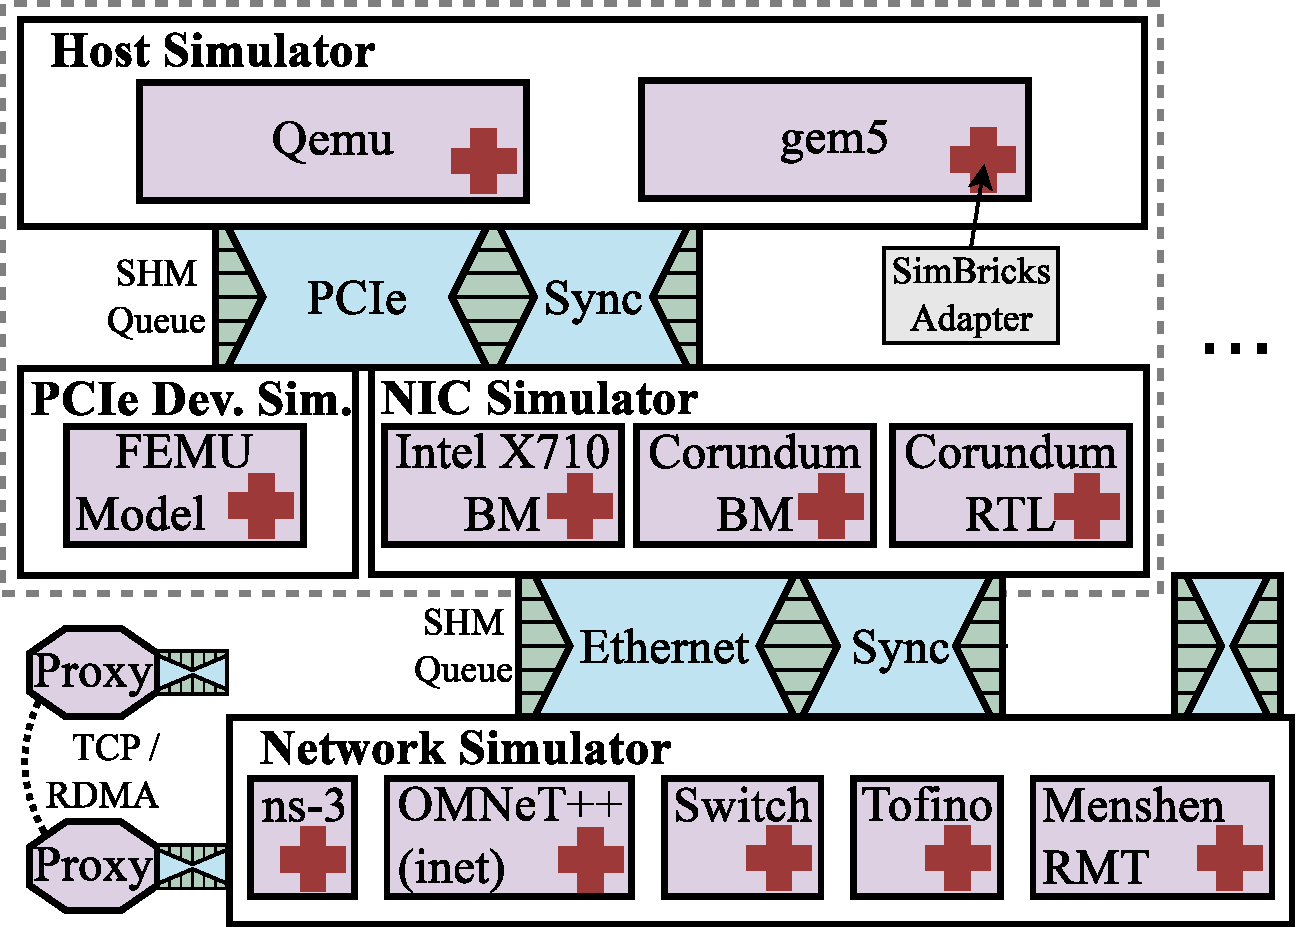
\includegraphics[width=0.4\textwidth]{figures/simarch.pdf}%
\caption{\sysname architecture.
\emph{Double hour glass} with narrow waists between hosts and
  devices, and NICs and networks.}%
\label{fig:sim-arch}%
\Description{Layered architecture diagram. At the two two layers
  grouped loosely: host simulators and PCIe device simulators.
  At the bottom the network simulator layers. host layers connect
  to PCIe device, some of the PCIe deices (NICs) connect to network
  simulators. These connections represented as narrow waists, are
  realized through shared memory queues. RDMA and TCP proxy pairs
  connect to these same connectors. Inside each layer the specific
  simulators along with a symbol indicating a \sysnet adapters are
  shown as boxes. Host simulators are: QEMU and gem5. PCIe devices
  are: the FEMU ssd model, and three NICs (Intel x710 behavioral
  model, Corundum behavioral model, and Corundum RTL simulation).
  Finally network simulators are: ns-3, OMNET++ (inet), switch,
  Tofino, and Menshen RMT.}%
\end{figure}


Using our design principles, we have built \sysname, a modular,
end-to-end simulation framework shown in \autoref{fig:sim-arch}.
%
In this section, we detail the design of \sysname{}, including
simulator interfaces, fast message transport, techniques to scale
up and out to larger simulations, and the synchronization mechanism.

\subsection{Component Simulator Interfaces}
\label{ssec:design:interface}
%
\sysname{} achieves modularity through well-defined interfaces
between component simulators:
%
Host simulators connect to device simulators through a PCIe interface;
%
NIC and network simulators interconnect through an
Ethernet interface.
%
This results in a double hourglass architecture
(\autoref{fig:sim-arch}) with narrow waists at component boundaries.
%
In physical systems both interfaces are asynchronous and incur
propagation delay ($\Delta_i$).
%
We replicate both aspects.


\begin{figure}[t]%
\centering%
\begin{minipage}{\linewidth}%
\centering%
\small%
\begin{tabular}{cl}
  \toprule[1.5pt]
    \multicolumn{2}{c}{\textbf{PCIe:} Device $\rightarrow$ Host} \\
    \textbf{Message Type} &
    \textbf{Message Fields} \\
  \midrule[1pt]
    \texttt{INIT\_DEV} &
    \begin{tabular}[c]{@{}l@{}}
      PCI vendor, device id, class, \\
      subclass, revision, \\
      \# of MSI vectors, \# of MSI-X vectors, \\
      table/PBA bar and offset
    \end{tabular} \\
  \midrule[0.5pt]
    \begin{tabular}[c]{@{}c@{}}
      \texttt{DMA\_READ},\\
      \texttt{DMA\_WRITE}\\
    \end{tabular} &
    \begin{tabular}[c]{@{}l@{}}
      request ID, memory address, length, \\
      payload data (optional)
    \end{tabular} \\
  \midrule[0.5pt]
    \texttt{MMIO\_COMPL} &
    request ID, payload data (optional) \\
  \midrule[0.5pt]
    \texttt{INTERRUPT} &
    \begin{tabular}[c]{@{}l@{}}
      interrupt type, \\
      MSI/MSI-X: vector \#, \\
      legacy: level
    \end{tabular} \\
  \midrule[0.5pt]
  %%%%%%%%%%%%%%%%%%%
  \midrule[1.5pt]
    \multicolumn{2}{c}{\textbf{PCIe:} Host $\rightarrow$ Device} \\
    \textbf{Message Type} &
    \textbf{Message Fields} \\
  \midrule[1pt]
    \texttt{DMA\_COMPL} &
    request ID, payload data (optional) \\
  \midrule[0.5pt]
    \begin{tabular}[c]{@{}c@{}}
      \texttt{MMIO\_READ}, \\
      \texttt{MMIO\_WRITE}
    \end{tabular} &
    \begin{tabular}[c]{@{}l@{}}
      request ID, BAR \# and offset, length, \\
      payload data (optional)
    \end{tabular} \\
  \midrule[0.5pt]
    \texttt{INT\_STATUS} &
    interrupts enabled: legacy, MSI, MSI-X \\
  \midrule[1.5pt] \\
  %%%%%%%%%%%%%%%%%%%
  \midrule[1.5pt]
    \multicolumn{2}{c}{\textbf{Ethernet:} NIC $\leftrightarrow$
    Net / Net $\leftrightarrow$ Net} \\
    \textbf{Message Type} &
    \textbf{Message Fields} \\
  \midrule[1pt]
    \texttt{PACKET} &
    \begin{tabular}[c]{@{}l@{}}
      packet length, packet data
    \end{tabular} \\
  \bottomrule[1.5pt]
\end{tabular}%
\end{minipage}%
\caption{\sysname's simulator interfaces: PCIe between host and
      device, and Ethernet between network components.}%
\label{fig:interface}%
\Description{Messages for the PCIe and Ethernet protocols in
\sysname. For PCIe the protocol is asymmetrical, while Ethernet is
symmetrical. For PCIe from the device to the host, the messages are:
INIT\_DEV (with PCI vendor, device, class, subclass, revision IDs, the
number of MSI and MSI-X vectors, and the MSI-X table and PBA bars and
offsets), DMA\_READ and DMA\_WRITE (with request ID, memory address,
length, and payload for write), MMIO\_COMPL (with request ID, payload
data for read), and INTERRUPT (interrupt type, MSI/MSI-X vector, or
legacy interrupt level). In the opposite direction, Host to device the
messages are: DMA\_COMPL (with request ID, payload data for reads),
MMIO\_READ and MMIO\_WRITE (with request ID, BAR number and offset,
length, payload data for writes), INT\_STATUS (with flags for enabled
interrupts: legacy, MSI, MSI-X). For Ethernet there is only one
message: PACKET (with length and packet data).}%
\end{figure}


\subsubsection{PCIe: Host-Device Interface}\hfill\\
PCIe itself is a layered protocol, ranging from the
low-level physical layer to the transactional layer for data
operations.
%
We define \sysname{}'s host-device interface (\autoref{fig:interface})
based on the PCIe \textit{transactional layer}, and abstract
away physical attributes of the PCIe link with simple parameters --
link bandwidth and latency.
%
Low-level complexity such as encoding and signaling are unnecessary
for most system simulations and would incur substantial cost and
complexity for each simulator.
%
Should future use-cases need to model this, a detailed PCIe simulator
could be integrated as an interposed component
(\autoref{ssec:design:decomp}).


\paragraph{Discovery and Initialization.}
A key PCIe feature is that hosts can enumerate and identify connected
devices and the features they support.
%
To this end, our interface defines the \texttt{INIT\_DEV} message for
registering device simulators with the host simulator.
%
The device simulator includes device information in the message, such as the PCI
vendor, device identifiers, base address registers (BARs), the number of MSI(-X)
interrupt vectors, and addresses of the MSI-X table and PBA.
%
The host simulator uses this information to expose a corresponding PCIe device
to the system.


\paragraph{Data transfers: MMIO \& DMA.}
PCIe data transfers are symmetrical: both sides can initiate reads
and writes, which the other side completes.
%
\sysname{}'s PCIe interface defines \texttt{DMA\_READ} /
\texttt{WRITE} messages for DMA transfers initiated by device
simulators, and \texttt{MMIO\_READ} / \texttt{WRITE} for MMIO accesses
initiated by host simulators.
%
As in PCIe, all data transfer operations are \textit{asynchronous}.
%
Once a request is finished, the device simulator issues a \texttt{MMIO\_COMPL}
completion message, while the host simulator adapter sends a
\texttt{DMA\_COMPL}.
%
PCIe allows multiple outstanding operations and only guarantees that
they will be issued to the memory system in the order of arrival.
%
Completion events, however, may arrive out-of-order.
%
To match completions with outstanding requests, all requests carry an
identifier that the receiving simulator includes in the response.

\paragraph{Interrupts.}
Our interface supports all PCIe interrupt signaling methods:
legacy interrupts (INTX), message signaled interrupts (MSI), and
MSI-X.
%
Physical PCIe devices implement MSI (including configuration,
masking, and generating signalling operations) completely on the
device side.
%
To reduce repeated implementation effort in device simulators and
integration challenges in host simulators, we instead opt to keep this
functionality inside the host simulator.
%
Device issues \texttt{INTERRUPT} messages to either trigger an
interrupt vector for MSI(-X) or to set interrupt pin state for INTX.
%
To support devices that require knowledge about which interrupt
mechanisms the OS has enabled,
our interface provides the \texttt{INT\_STATUS} message which the host simulator
sends on configuration changes.



\subsubsection{Ethernet: Network Component Interface} \hfill\\
\label{sssec:design:interface:nicnet}
In \sysname{}'s network interface, we similarly abstract away
low-level details of the Ethernet standard, and only expose Ethernet
frames, as \texttt{PACKET} messages, to NIC and network
simulators.
%
A \texttt{PACKET} message carries the length of the packet alongside
packet payload, but omits CRCs to reduce overhead as none of our
network simulators models them and most NICs strip them after
validation.
%
If future network or NIC simulators require CRCs, their \sysname adapter can
transparently generate and strip the checksums, as we currently do not model
data corruption.
%
We leave support for hardware flow control as future work.




\subsection{Inter-Simulator Message Transport}
\label{ssec:design:transport}
\sysname runs component simulators as separate processes communicating
through message passing.
%
Thus, efficient inter-process communication is critical for the overall
performance.
%
We use optimized shared memory queues with polling for efficient
message transport between simulators.
%
For parallel processes on separate cores, shared memory queues
enable low-latency communication with minimal
overhead~\cite{bershad:urpc,baumann:barrelfish}.
%
Between any pair of \emph{communicating} simulators, \sysname
establishes a bidirectional message channel consisting of a pair of
unidirectional queues in opposite directions.
%
During channel initialization, \sysname uses a Unix socket to provide a named
endpoint for connection setup and for communicating queue parameters and shared
memory file descriptors.

\sysname uses concurrent, circular, single-producer and consumer queues.
%
They comprise an array of fixed-sized, cache line aligned message
slots.
%
The last byte in each slot is reserved for metadata:
one bit indicating the current owner of the slot (\texttt{consumer} or
\texttt{producer}) and the rest for the message type.
%
As queues are single-producer and single-consumer, we store the tail pointer
\textit{locally} at the producer and the head pointer at the consumer.
%
Consumers poll for a message in the next slot, until the ownership
flag indicates \texttt{consumer}.
%
After processing the message the consumer resets the ownership flag.
%
Producers similarly wait for the next slot to be available, fill it,
and switch the ownership flag.


The \sysname message transport design avoids cache coherence overhead unless it
is fundamentally necessary.
%
Since head and tail pointers are local to consumer and producer
respectively, only accesses to shared message slots result in
coherence traffic.
%
Moreover, as long as a consumer does not poll in between the producer
writing a message to the corresponding slot and setting the ownership
bit, all coherence traffic carries necessary data from producer to
consumer~\cite{baumann:barrelfish}.
We include additional detail and pseudocode in \autoref{sec:appendix:shm}.


\subsection{Scaling Up with Decomposition}
\label{ssec:design:decomp}
\sysname can scale to larger simulations by adding more component simulators.
%
For instance, a network simulator connecting to many devices may become a
bottleneck as it needs to synchronize with all peers.
%
We leverage the \sysname architecture to improve scalability, by
decomposing the network simulator into multiple processes that
connect and synchronize via \sysname Ethernet interfaces.
%
Other simulators, such as a gem5 simulated host, can be accelerated in a similar
fashion by decomposing into connected components.
%
We will demonstrate the scalability benefit of our decomposition approach in
\autoref{ssec:eval:scalability}.


\subsection{Scaling Out with Proxies}
\label{ssec:design:proxy}
Running simulators in parallel on dedicated cores maximizes parallelism, but the
number of available cores in a single machine limits simulation size.
%
Message passing and modular simulation in \sysname enables us to scale out
simulations by partitioning components to multiple hosts and replacing message
queues between simulators on different hosts with network communication.
%
However, directly implementing this in individual component simulators
has two major drawbacks.
%
First, it increases the complexity for integration,
as each simulator adapter needs to implement an additional message
transport.
%
Second, it increases communication overhead in component simulators,
leaving fewer processor cycles for simulators and increasing
simulation time.
%
To avoid these drawbacks, we instead implement network communication
in proxies.
%
\sysname proxies connect to local component simulators through
existing shared memory queues and forward messages over the network to
their peer proxy which operates symmetrically.
%
This requires an additional processor core for the proxy on each side,
but is fully transparent to component simulators and does not increase
their communication overhead.



\subsection{Simulator Synchronization Mechanism}
\label{ssec:design:syncproto}

To ensure accurate interconnection of component simulators, we design a
synchronization mechanism that that guarantees correctness while minimizing
overhead, even when scaling to large simulations.

\subsubsection{Naive Synchronization Mechanisms do not Scale} \hfill\\
A conceptual straw-man for synchronizing components are global
barriers at each time step, keeping simulators in lockstep.
%
When components are connected by communication links with non-zero
latency, frequency of global barriers can be reduced by dividing
simulation time into \textit{epochs} no larger than the lowest link
latency.
%
Global barriers are only required at epoch boundaries, since all
cross-component events will be delivered after the end of the
current epoch~\cite{reinhardt:wwt,mohammad:distgem5,alian:pd-gem5}.
%
Unfortunately, epoch-based synchronization still relies on
non-scalable global barriers across all simulators, with the barrier
frequency determined by the lowest link latency in the whole
simulation, incurring substantial synchronization overhead.

\subsubsection{Scalable synchronization in \sysname} \hfill\\
We avoid global synchronization while \textit{guaranteeing accurate
simulator interconnection} by relying on properties specific to the
\sysname architecture.
%
\autoref{fig:sync-proto} shows pseudocode for the \sysname
synchronization protocol.


\paragraph{Enforcing message processing times is sufficient.}
In \sysname, all communication between simulators is explicit through
message passing along statically created point-to-point channels.
%
Thus, the only requirement for accurate simulation is that
\emph{messages are processed at the correct
time}~\cite{chandy:distsim,bryant:distsim}.
%
Additional synchronization does not affect the simulation, as
simulators cannot otherwise observe or influence each other.
%
To enforce this guarantee, senders tag messages with the time when
the receiver must process the message.
%
For determinism, simulators with multiple peers must order messages with
identical timestamps consistently.

\paragraph{Pairwise synchronization is sufficient.}
All \sysname message passing channels are point-to-point and
statically determined by the simulation structure.
%
This is where we differ from most prior synchronization schemes:
they do not assume a known topology and thus require global
synchronization.
%
\sysname only needs to implement pairwise synchronization, between each
simulator and its a priori known peers~\cite{bryant:distsim}.

\paragraph{Per-channel message timestamps are monotonic.}
Our message queues deliver messages strictly in order.
%
Since each \sysname connection between two simulators incurs a
propagation latency $\Delta_i > 0$, a message sent at time
$T$ over interface $i$ arrives at $T + \Delta_i$.
%
Assuming simulator clocks advance monotonically,
message timestamps on each channel are thus monotonic.

\paragraph{Message timestamps ensure correctness.}
A corollary of monotonic timestamps is that
a message with timestamp $t$ is an implicit promise that no
messages with timestamps $<t$ will arrive on that channel later.
%
Therefore, once a simulator receives messages with timestamps
$\ge T$ from \emph{all} its peers, it can safely advance
its clock to $T$ without more coordination.



\paragraph{Ensuring liveness with sync messages.}
The above conditions ensure accuracy, but do not guarantee liveness.
%
Simulations can only make progress when every channel carries at
least one message in each direction in every $\Delta_i$ time
interval~\cite{chandy:distsim,bryant:distsim}.
%
To ensure progress, we introduce \texttt{SYNC} messages that
simulators send if they have not sent any messages for
$\delta_i \le \Delta_i$ time units.
%
\texttt{SYNC} messages allow connected peers to advance their clocks in the
absence of data messages.
%
In our simulations we set $\delta_i = \Delta_i$;
%
lower values of $\delta_i$ are valid, but we have not found
configurations where the benefit of more frequent clock advances
outweighed the cost of sending and processing additional
\texttt{SYNC} messages.

\paragraph{Link latency provides synchronization slack.}
Non-zero link latencies further reduce synchronization overhead, since
not even peer simulators need to execute in lockstep.
%
Specifically, a message sent at $T$ allows its peer to advance to $T +
\Delta_i$.
%
At that point, the peer's clock is guaranteed to lay between $T -
\Delta_i$ (otherwise the local clock would not be at $T$) and
$T + \Delta_i$.
%
Different channels in a \sysname configuration can use different
$\Delta_i$ values.
%
While synchronized simulations are fundamentally only as fast as the
slowest component, this slack improves efficiency by absorbing small
transient variation in simulation speed, without immediately blocking
all simulators.

\begin{figure}%
  \begin{minipage}{\linewidth}
  %\vspace{-1em}%
  \begin{algorithmic}[0]%
    \Procedure{Init}{}
      \For{if \textbf{in} interfaces}
        \State \Call{SyncTimer}{if}
        \State msg $\gets$ \Call{PollMsg}{if}
        \State \Call{Reschedule}{msg.timestamp, \textsc{RxTimer}, msg, if}
      \EndFor
    \EndProcedure
    \Procedure{SyncTimer}{if}
      \State msg $\gets$ \Call{AllocMsg}{if}
      \State msg.type $\gets$ \texttt{SYNC}
      \State \Call{SendMsg}{msg}
    \EndProcedure
    \Procedure{RxTimer}{msg, if}
      \If{msg.type $\ne$ \texttt{SYNC}}
        \State \Call{ProcessMsg}{msg}
      \EndIf
      \State msg $\gets$ \Call{PollMsg}{if}
      \State \Call{Reschedule}{msg.timestamp, \textsc{RxTimer}, msg, if}
    \EndProcedure
    \Procedure{SendMsg}{msg, if}
      \State msg.timestamp $\gets T + \Delta_{\textrm{if}}$
      \State \Call{EnqueueMsg}{msg, if}
      \State \Call{Reschedule}{$T + \delta_{\textrm{if}}$, \textsc{SyncTimer}}
    \EndProcedure
  \end{algorithmic}%
\end{minipage}%
\caption{\sysname synchronization protocol pseudocode for a
    discrete event-based simulator.
    \textsc{Reschedule} schedules a callback for the specified time,
    cancelling earlier instances.
    \textsc{ProcessMsg} and \textsc{SendMsg} interface with the
    upper layer PCI or Network protocol. $\Delta_\textrm{if}$ is the
    link latency and $\delta_\textrm{if}$ the synchronization
    interval.}%
\label{fig:sync-proto}%
\Description{This figure shows pseudo-code but the text is included as
  in the PDF and as such should be accessible.}%
\end{figure}


